%
% This is an example LaTeX file which uses the SANDreport class file.
% It shows how a SAND report should be formatted, what sections and
% elements it should contain, and how to use the SANDreport class.
% It uses the LaTeX article class, but not the strict option.
% ItINLreport uses .eps logos and files to show how pdflatex can be used
%
% Get the latest version of the class file and more at
%    http://www.cs.sandia.gov/~rolf/SANDreport
%
% This file and the SANDreport.cls file are based on information
% contained in "Guide to Preparing {SAND} Reports", Sand98-0730, edited
% by Tamara K. Locke, and the newer "Guide to Preparing SAND Reports and
% Other Communication Products", SAND2002-2068P.
% Please send corrections and suggestions for improvements to
% Rolf Riesen, Org. 9223, MS 1110, rolf@cs.sandia.gov
%
\documentclass[pdf,12pt]{../../user_manual/INLreport}
% pslatex is really old (1994).  It attempts to merge the times and mathptm packages.
% My opinion is that it produces a really bad looking math font.  So why are we using it?
% If you just want to change the text font, you should just \usepackage{times}.
% \usepackage{pslatex}
\usepackage{times}
\usepackage{longtable}
\usepackage[FIGBOTCAP,normal,bf,tight]{subfigure}
\usepackage{amsmath}
\usepackage{amssymb}
\usepackage[labelfont=bf]{caption}
\usepackage{pifont}
\usepackage{enumerate}
\usepackage{listings}
\usepackage{fullpage}
\usepackage{xcolor}          % Using xcolor for more robust color specification
\usepackage{ifthen}          % For simple checking in newcommand blocks
\usepackage{textcomp}
%\usepackage{authblk}         % For making the author list look prettier
%\renewcommand\Authsep{,~\,}

% Custom colors
\definecolor{deepblue}{rgb}{0,0,0.5}
\definecolor{deepred}{rgb}{0.6,0,0}
\definecolor{deepgreen}{rgb}{0,0.5,0}
\definecolor{forestgreen}{RGB}{34,139,34}
\definecolor{orangered}{RGB}{239,134,64}
\definecolor{darkblue}{rgb}{0.0,0.0,0.6}
\definecolor{gray}{rgb}{0.4,0.4,0.4}

\lstset {
  basicstyle=\ttfamily,
  frame=single
}

\setcounter{secnumdepth}{5}
\lstdefinestyle{XML} {
    language=XML,
    extendedchars=true,
    breaklines=true,
    breakatwhitespace=true,
%    emph={name,dim,interactive,overwrite},
    emphstyle=\color{red},
    basicstyle=\ttfamily,
%    columns=fullflexible,
    commentstyle=\color{gray}\upshape,
    morestring=[b]",
    morecomment=[s]{<?}{?>},
    morecomment=[s][\color{forestgreen}]{<!--}{-->},
    keywordstyle=\color{cyan},
    stringstyle=\ttfamily\color{black},
    tagstyle=\color{darkblue}\bf\ttfamily,
    morekeywords={name,type},
%    morekeywords={name,attribute,source,variables,version,type,release,x,z,y,xlabel,ylabel,how,text,param1,param2,color,label},
}
\lstset{language=python,upquote=true}

\usepackage{titlesec}
\newcommand{\sectionbreak}{\clearpage}
\setcounter{secnumdepth}{4}

%\titleformat{\paragraph}
%{\normalfont\normalsize\bfseries}{\theparagraph}{1em}{}
%\titlespacing*{\paragraph}
%{0pt}{3.25ex plus 1ex minus .2ex}{1.5ex plus .2ex}

%%%%%%%% Begin comands definition to input python code into document
\usepackage[utf8]{inputenc}

% Default fixed font does not support bold face
\DeclareFixedFont{\ttb}{T1}{txtt}{bx}{n}{9} % for bold
\DeclareFixedFont{\ttm}{T1}{txtt}{m}{n}{9}  % for normal

\usepackage{listings}

% Python style for highlighting
\newcommand\pythonstyle{\lstset{
language=Python,
basicstyle=\ttm,
otherkeywords={self, none, return},             % Add keywords here
keywordstyle=\ttb\color{deepblue},
emph={MyClass,__init__},          % Custom highlighting
emphstyle=\ttb\color{deepred},    % Custom highlighting style
stringstyle=\color{deepgreen},
frame=tb,                         % Any extra options here
showstringspaces=false            %
}}


% Python environment
\lstnewenvironment{python}[1][]
{
\pythonstyle
\lstset{#1}
}
{}

% Python for external files
\newcommand\pythonexternal[2][]{{
\pythonstyle
\lstinputlisting[#1]{#2}}}

\lstnewenvironment{xml}
{}
{}

% Python for inline
\newcommand\pythoninline[1]{{\pythonstyle\lstinline!#1!}}

% Named Colors for the comments below (Attempted to match git symbol colors)
\definecolor{RScolor}{HTML}{8EB361}  % Sonat (adjusted for clarity)
\definecolor{DPMcolor}{HTML}{E28B8D} % Dan
\definecolor{JCcolor}{HTML}{82A8D9}  % Josh (adjusted for clarity)
\definecolor{AAcolor}{HTML}{8D7F44}  % Andrea
\definecolor{CRcolor}{HTML}{AC39CE}  % Cristian
\definecolor{RKcolor}{HTML}{3ECC8D}  % Bob (adjusted for clarity)
\definecolor{DMcolor}{HTML}{276605}  % Diego (adjusted for clarity)
\definecolor{PTcolor}{HTML}{990000}  % Paul

\def\DRAFT{} % Uncomment this if you want to see the notes people have been adding
% Comment command for developers (Should only be used under active development)
\ifdefined\DRAFT
  \newcommand{\nameLabeler}[3]{\textcolor{#2}{[[#1: #3]]}}
\else
  \newcommand{\nameLabeler}[3]{}
\fi
\newcommand{\alfoa}[1] {\nameLabeler{Andrea}{AAcolor}{#1}}
\newcommand{\cristr}[1] {\nameLabeler{Cristian}{CRcolor}{#1}}
\newcommand{\mandd}[1] {\nameLabeler{Diego}{DMcolor}{#1}}
\newcommand{\maljdan}[1] {\nameLabeler{Dan}{DPMcolor}{#1}}
\newcommand{\cogljj}[1] {\nameLabeler{Josh}{JCcolor}{#1}}
\newcommand{\bobk}[1] {\nameLabeler{Bob}{RKcolor}{#1}}
\newcommand{\senrs}[1] {\nameLabeler{Sonat}{RScolor}{#1}}
\newcommand{\talbpaul}[1] {\nameLabeler{Paul}{PTcolor}{#1}}
% Commands for making the LaTeX a bit more uniform and cleaner
\newcommand{\TODO}[1]    {\textcolor{red}{\textit{(#1)}}}
\newcommand{\xmlAttrRequired}[1] {\textcolor{red}{\textbf{\texttt{#1}}}}
\newcommand{\xmlAttr}[1] {\textcolor{cyan}{\textbf{\texttt{#1}}}}
\newcommand{\xmlNodeRequired}[1] {\textcolor{deepblue}{\textbf{\texttt{<#1>}}}}
\newcommand{\xmlNode}[1] {\textcolor{darkblue}{\textbf{\texttt{<#1>}}}}
\newcommand{\xmlString}[1] {\textcolor{black}{\textbf{\texttt{'#1'}}}}
\newcommand{\xmlDesc}[1] {\textbf{\textit{#1}}} % Maybe a misnomer, but I am
                                                % using this to detail the data
                                                % type and necessity of an XML
                                                % node or attribute,
                                                % xmlDesc = XML description
\newcommand{\default}[1]{~\\*\textit{Default: #1}}
\newcommand{\nb} {\textcolor{deepgreen}{\textbf{~Note:}}~}

%%%%%%%% End comands definition to input python code into document

%\usepackage[dvips,light,first,bottomafter]{draftcopy}
%\draftcopyName{Sample, contains no OUO}{70}
%\draftcopyName{Draft}{300}

% The bm package provides \bm for bold math fonts.  Apparently
% \boldsymbol, which I used to always use, is now considered
% obsolete.  Also, \boldsymbol doesn't even seem to work with
% the fonts used in this particular document...
\usepackage{bm}

% Define tensors to be in bold math font.
\newcommand{\tensor}[1]{{\bm{#1}}}

% Override the formatting used by \vec.  Instead of a little arrow
% over the letter, this creates a bold character.
\renewcommand{\vec}{\bm}

% Define unit vector notation.  If you don't override the
% behavior of \vec, you probably want to use the second one.
\newcommand{\unit}[1]{\hat{\bm{#1}}}
% \newcommand{\unit}[1]{\hat{#1}}

% Use this to refer to a single component of a unit vector.
\newcommand{\scalarunit}[1]{\hat{#1}}

% \toprule, \midrule, \bottomrule for tables
\usepackage{booktabs}

% \llbracket, \rrbracket
\usepackage{stmaryrd}

\usepackage{hyperref}
\hypersetup{
    colorlinks,
    citecolor=black,
    filecolor=black,
    linkcolor=black,
    urlcolor=black
}

\newcommand{\wiki}{\href{https://github.com/idaholab/raven/wiki}{RAVEN wiki}}

% Compress lists of citations like [33,34,35,36,37] to [33-37]
\usepackage{cite}

% If you want to relax some of the SAND98-0730 requirements, use the "relax"
% option. It adds spaces and boldface in the table of contents, and does not
% force the page layout sizes.
% e.g. \documentclass[relax,12pt]{SANDreport}
%
% You can also use the "strict" option, which applies even more of the
% SAND98-0730 guidelines. It gets rid of section numbers which are often
% useful; e.g. \documentclass[strict]{SANDreport}

% The INLreport class uses \flushbottom formatting by default (since
% it's intended to be two-sided document).  \flushbottom causes
% additional space to be inserted both before and after paragraphs so
% that no matter how much text is actually available, it fills up the
% page from top to bottom.  My feeling is that \raggedbottom looks much
% better, primarily because most people will view the report
% electronically and not in a two-sided printed format where some argue
% \raggedbottom looks worse.  If we really want to have the original
% behavior, we can comment out this line...
\raggedbottom
\setcounter{secnumdepth}{5} % show 5 levels of subsection
\setcounter{tocdepth}{5} % include 5 levels of subsection in table of contents

% ---------------------------------------------------------------------------- %
%
% Set the title, author, and date
%
\title{RAVEN Software Design Description}
%\author{%
%\begin{tabular}{c} Author 1 \\ University1 \\ Mail1 \\ \\
%Author 3 \\ University3 \\ Mail3 \end{tabular} \and
%\begin{tabular}{c} Author 2 \\ University2 \\ Mail2 \\ \\
%Author 4 \\ University4 \\ Mail4\\
%\end{tabular} }


\author{Andrea Alfonsi}
 

% There is a "Printed" date on the title page of a SAND report, so
% the generic \date should [WorkingDir:]generally be empty.
\date{}


% ---------------------------------------------------------------------------- %
% Set some things we need for SAND reports. These are mandatory
%
\SANDnum{SDD-513}
\SANDprintDate{December  2018}
\SANDauthor{Andrea Alfonsi}
\SANDreleaseType{Revision 0}

% ---------------------------------------------------------------------------- %
% Include the markings required for your SAND report. The default is "Unlimited
% Release". You may have to edit the file included here, or create your own
% (see the examples provided).
%
% \include{MarkOUO} % Not needed for unlimted release reports

\def\component#1{\texttt{#1}}

% ---------------------------------------------------------------------------- %
\newcommand{\systemtau}{\tensor{\tau}_{\!\text{SUPG}}}

% Added by Sonat
\usepackage{placeins}
\usepackage{array}

\newcolumntype{L}[1]{>{\raggedright\let\newline\\\arraybackslash\hspace{0pt}}m{#1}}
\newcolumntype{C}[1]{>{\centering\let\newline\\\arraybackslash\hspace{0pt}}m{#1}}
\newcolumntype{R}[1]{>{\raggedleft\let\newline\\\arraybackslash\hspace{0pt}}m{#1}}

% end added by Sonat
% ---------------------------------------------------------------------------- %
%
% Start the document
%

\begin{document}
    \maketitle

    % ------------------------------------------------------------------------ %
    % An Abstract is required for SAND reports
    %
%    \begin{abstract}
%    \input abstract
%    \end{abstract}


    % ------------------------------------------------------------------------ %
    % An Acknowledgement section is optional but important, if someone made
    % contributions or helped beyond the normal part of a work assignment.
    % Use \section* since we don't want it in the table of context
    %
%    \clearpage
%    \section*{Acknowledgment}



%	The format of this report is based on information found
%	in~\cite{Sand98-0730}.


    % ------------------------------------------------------------------------ %
    % The table of contents and list of figures and tables
    % Comment out \listoffigures and \listoftables if there are no
    % figures or tables. Make sure this starts on an odd numbered page
    %
    \cleardoublepage		% TOC needs to start on an odd page
    \tableofcontents
    %\listoffigures
    %\listoftables


    % ---------------------------------------------------------------------- %
    % An optional preface or Foreword
%    \clearpage
%    \section*{Preface}
%    \addcontentsline{toc}{section}{Preface}
%	Although muggles usually have only limited experience with
%	magic, and many even dispute its existence, it is worthwhile
%	to be open minded and explore the possibilities.


    % ---------------------------------------------------------------------- %
    % An optional executive summary
    %\clearpage
    %\section*{Summary}
    %\addcontentsline{toc}{section}{Summary}
    %\input{Summary.tex}
%	Once a certain level of mistrust and skepticism has
%	been overcome, magic finds many uses in todays science



%	and engineering. In this report we explain some of the
%	fundamental spells and instruments of magic and wizardry. We
%	then conclude with a few examples on how they can be used
%	in daily activities at national Laboratories.


    % ---------------------------------------------------------------------- %
    % An optional glossary. We don't want it to be numbered
%    \clearpage
%    \section*{Nomenclature}
%    \addcontentsline{toc}{section}{Nomenclature}
%    \begin{description}
%          \item[alohomoral]
%           spell to open locked doors and containers
%          \item[leviosa]
%           spell to levitate objects
%    \item[remembrall]
%           device to alert you that you have forgotten something
%    \item[wand]
%           device to execute spells
%    \end{description}


    % ---------------------------------------------------------------------- %
    % This is where the body of the report begins; usually with an Introduction
    %
    \SANDmain		% Start the main part of the report

\section{Introduction}
\subsection{System Purpose}

RAVEN is a flexible and multi-purpose uncertainty quantification (UQ), regression analysis, probabilistic risk assessment 
(PRA), data analysis and model optimization software.  Depending on the tasks to be accomplished and on the 
probabilistic
 characterization of the problem, RAVEN perturbs (Monte-Carlo, latin hyper-cube, reliability surface search, etc.) the
 response of the system under consideration by altering its own parameters. The system is modeled by third party
 software (RELAP5-3D, MAAP5, BISON, etc.) and accessible to RAVEN either directly (software coupling) or
 indirectly (via input/output files). The data generated by the sampling process is analyzed using classical statistical
 and more advanced data mining approaches. RAVEN also manages the parallel dispatching (i.e. both on
 desktop/workstation and large High-Performance Computing machines) of the software representing the physical 
 model. RAVEN heavily relies on artificial intelligence algorithms to construct surrogate models of complex physical
 systems in order to perform uncertainty quantification, reliability analysis (limit state surface) and parametric studies.

\subsection{System Scope}

RAVEN’s scope is to provide a set of capabilities to build analysis flows based on UQ, PRA, Optimization and Data Analysis techniques to be applied to any physical model(s). The main objective of the software is to assist the engineer/user to:
\begin{itemize}
  \item identify the best design (on any physics/model), its safety and confidence;
  \item estimate the likelihood of undesired outcomes (risk analysis);
  \item identify main drivers/events to act on for reducing impact/consequences of anomalous dynamic behaviors of the 
         system under analysis;
  \item to construct analysis flows combining multiple physical models and analysis procedures.
\end{itemize}

In other words, the RAVEN software is aimed to be employed for:
\begin{itemize}
  \item Uncertainty Quantification;
  \item Sensitivity Analysis / Regression Analysis;
  \item Probabilistic Risk and Reliability Analysis (PRA);
  \item Data Mining Analysis;
  \item Model Optimization.
\end{itemize}

The combination of all the previously mentioned analysis capabilities is a key component to 
define safety margins in engineering design that are more representative of real prediction deficiencies. 
This could reduce 
cost and maintain a more coherent safety level of the system (no excess/no lack of safety margins in any operational 
condition).
The risk analysis, assisted by the data mining algorithms, is used to find engineering solutions to reduce costs, while 
preserving safety margins, or to increase safety at the minimum cost. These tasks can be automatically achieved by using 
optimization algorithms available in the RAVEN software.
Moreover, the knowledge of the relationship between input and system response uncertainties allows identifying effective 
experiments, which are the most suitable for increasing the accuracy of the model. This approach reduces time and cost 
of the deployment of complex engineering systems and new technologies.

The RAVEN software employs several novel and unique techniques, based on extensive usage of artificial intelligence 
algorithms, such as adaptive (smart) sampling, adaptive branching algorithms (Dynamic Event Tree), time-dependent 
statistical analysis and data mining. 
The overall set of algorithms implemented in the RAVEN software are designed to handle highly non-linear systems, 
characterized by system response discontinuities and discrete variables. These capabilities are crucial for handling 
complex system models, such as nuclear power plants.
For example, reliability surface analysis, as implemented in RAVEN, is unique and capable to handle non-linear, 
discontinuous systems, allowing for faster and more accurate assessing of failure risk for complex systems.

In addition, the RAVEN software provides the unique capability to combine any model (e.g. physical models, surrogate 
models, data analysis models, etc.) in a single entity (named Ensemble Model) where each model can feedback into others. This capability allows the user to analyze system that could be simulated only by using complex computational work-flows.

\subsection{User Characteristics}

The users of the RAVEN software are expected to be part of any of the
following categories:
\begin{itemize}
  \item \textbf{Core developers (RAVEN core team)}: These are the developers of the RAVEN software. They will be responsible for following
    and enforcing the appropriate software development standards. They will be responsible for designing, implementing and 
    maintaining the software.
  \item \textbf{External developers}: A Scientist or Engineer that utilizes the RAVEN framework and wants to extend its capabilities (new interface to external
 applications, new data analysis tecniques, new sampling strategies, etc).This user will typically have a background in modeling and 
simulation techniques and/or numerical analysis but may only have a limited skill-set when it comes to object-oriented coding, C++/Python languages.
  \item \textbf{Analysts}:  These are users that will run the code and perform various analysis on the simulations they perform. These users may interact with developers of the system requesting new features and reporting bugs found and will typically make heavy use of the input file format.
\end{itemize}

\subsection{Other Design Documentation}

In addition to this document, an automatic software documentation
is generated every time a new CR (see def.) is approved. This
documentation is automatically extracted from the source code using
doxygen (see def.) and is available to developers at
\url{https://hpcsc.inl.gov/ssl/RAVEN/docs/classes.html}.

In order to generate(locally) a hard copy in ``html'' or ``latex'', any user/developer can 
launch the 
following command (in the raven directory):
\begin{lstlisting}[language=bash]
doxygen ./doc/doxygen/Doxyfile
\end{lstlisting}
Once the documentation is generated, any user/developer can navigate to the folder
\begin{lstlisting}[language=bash]
./doc/doxygen/latex
\end{lstlisting}
and type the following command:
\begin{lstlisting}[language=bash]
make refman.pdf
\end{lstlisting}
Once the command is executed, a ``pdf'' file named ``refman.pdf'' will be available.

The doxygen software is under configuration management process identified in
`` RAVEN Configuration Management '' PLN-5553.

\subsection{Dependencies and Limitations}
The software should be designed with the fewest possible constraints. 
Ideally the software should run on a wide variety of evolving hardware, 
so it should follow well-adopted standards and guidelines. The software
 should run on any POSIX compliant system (including Windows POSIX 
 emulators such as MinGW). The software will also make use of artificial 
 intelligence and numerical libraries that run on POSIX systems as well. 
 The main interface for the software will be command line based with no 
 assumptions requiring advanced terminal capabilities such as coloring and line control. 
 \\In order to be functional, RAVEN depends on the following software/libraries.
\begin{itemize}
  \item h5py-2.7.1
  \item numpy-1.12.1
  \item scipy-1.1.0
  \item scikit-learn-0.19.1
  \item pandas-0.20.3
  \item xarray-0.10.3
  \item netcdf4-1.4.0
  \item matplotlib-2.1.1
  \item statsmodels-0.8.0
  \item python-2.7
  \item hdf5-1.8.18
  \item swig
  \item pylint
  \item coverage
  \item lxml
  \item psutil
  \item pyside
  \item pillow
\end{itemize}

In addition, RAVEN (for its automatic regression test system), depends on MOOSE software (no libMesh or PTSC required).

\section{References}

\begin{itemize}

  \item ASME NQA 1 2008 with the NQA-1a-2009 addenda, ``Quality Assurance Requirements for Nuclear Facility Applications,'' First Edition, August 31, 2009.
  \item ISO/IEC/IEEE 24765:2010(E), ``Systems and software engineering Vocabulary,'' First Edition, December 15, 2010.
  \item LWP 13620, ``Managing Information Technology Assets''
\end{itemize}


\section{Definitions and Acronyms}

\subsection{Definitions}
\begin{itemize}
  \item \textbf{Baseline.} A specification or product (e.g., project plan, maintenance and operations [M\&O] plan, requirements, or 
design) that has been formally reviewed and agreed upon, that thereafter serves as the basis for use and further 
development, and that can be changed only by using an approved change control process. [ASME NQA-1-2008 with the 
NQA-1a-2009 addenda edited]
  \item \textbf{Validation.} Confirmation, through the provision of objective evidence (e.g., acceptance test), that the requirements 
for a specific intended use or application have been fulfilled. [ISO/IEC/IEEE 24765:2010(E) edited]
  \item \textbf{Verification.}
  \begin{itemize}
     \item The process of evaluating a system or component to determine whether the products of a given development 
     phase satisfy the conditions imposed at the start of that phase.
     \item  Formal proof of program correctness (e.g., requirements, design, implementation reviews, system tests). 
     [ISO/IEC/IEEE 24765:2010(E) edited]
  \end{itemize}
\end{itemize}

\subsection{Acronyms}
\begin{description}
\item[API] Application Programming Interfaces
\item[ASME] American Society of Mechanical Engineers
\item[CDF]  Comulative Distribution Functions
\item[DET] Dynamic Event Tree
\item[DOE] Department of Energy
\item[HDF5] Hierarchical Data Format (5)
\item[LWRS] Light Water Reactor Sustainability
\item[NEAMS] Nuclear Energy Advanced Modeling and Simulation
\item[NHES] Nuclear-Renewable Hybrid Energy Systems 
\item[INL] Idaho National Laboratory
\item[IT] Information Technology
\item[M\&O] Maintenance and Operations
\item[MC] Monte Carlo
\item[MOOSE] Multiphysics Object Oriented Simulation Environment
\item[NQA] Nuclear Quality Assurance
\item[POSIX]  Portable Operating System Interface
\item[PDF]  Probability Distribution (Density) Functions
\item[PP]  Post-Processor
\item[PRA]  Probabilistic Risk Assessment
\item[QA] Quality Assurance
\item[RAVEN] Risk Analysis and Virtual ENviroment
\item[ROM] Reduced Order Model
\item[SDD] System Design Description
\item[XML] eXtensible Markup Language 
\end{description}
\section{Design Stakeholders and Concerns}
\subsection{Design Stakeholders}
\begin{itemize}
  \item Light Water Reactor Sustainability (LWRS) program 
  \item Nuclear Energy Advanced Modeling and Simulation Program (NEAMS)
  \item Nuclear-Renewable Hybrid Energy Systems (NHES)
  \item Open-source community 
\end{itemize}
\subsection{Stakeholder Design Concerns}
The design of the RAVEN software in terms of functionality and capabilities to be deployed has been performed in 
accordance with the funding programs reported above. No specific concerns have been raised during the design and 
deployment of the RAVEN software. 

\section{Software Design}
\subsection{Introduction}
The Risk Analysis and Virtual ENviroment (RAVEN) mission is to provide a framework/container of capabilities for 
engineers and scientists to analyze the response of systems, physics and multi-physics, employing advanced numerical
techniques and algorithms.
RAVEN was conceived with two major objectives: 
\begin{itemize}
  \item  to be as easy and straightforward to use by scientists and engineers as possible. 
  \item to allow its expansion in a straightforward manner, providing clear and modular APIs  to developers.
\end{itemize}

The RAVEN software is meant to be approachable by any type of user (computational scientists, engineers and analysts). 
Every single aspect of RAVEN was driven by this singular principle from the build system to the APIs to the software development cycle and input syntax.

\begin{figure}[ht]
  \centering
  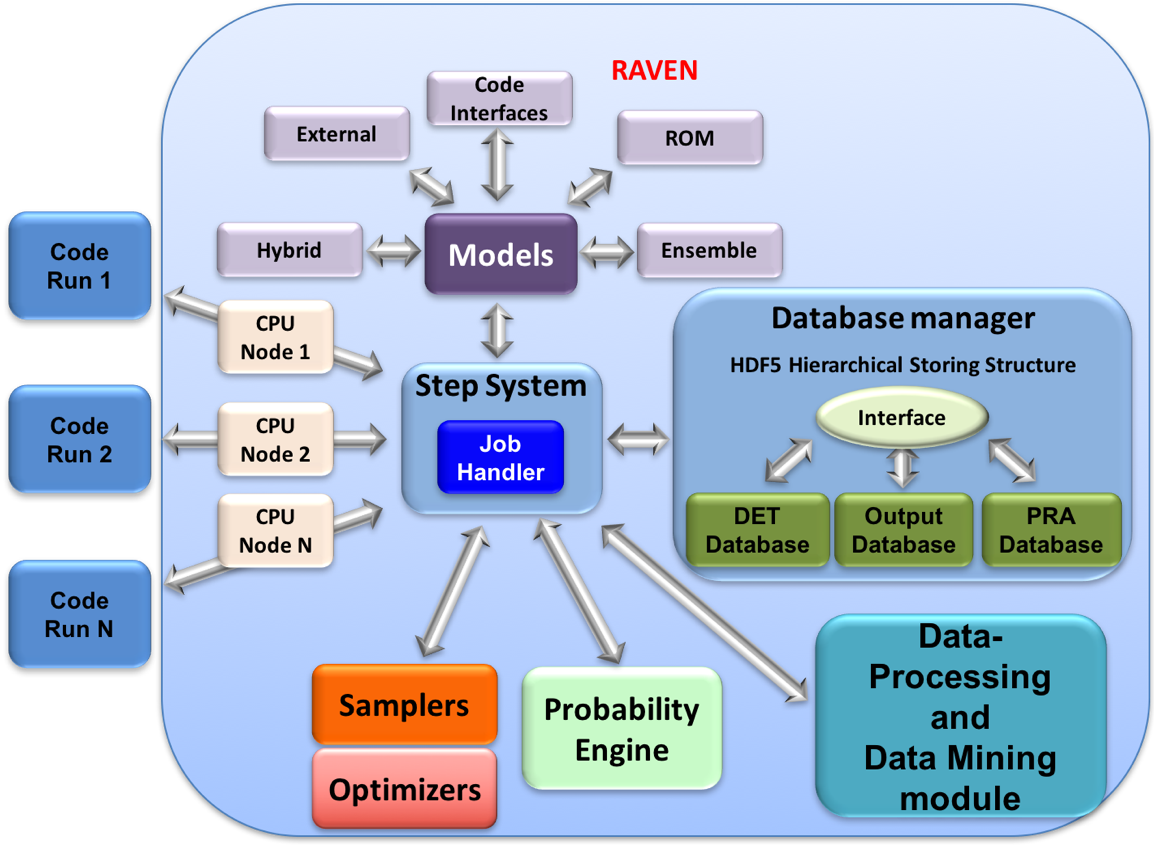
\includegraphics[width=0.9\textwidth]  {pics/RavenFramework.png}
  \caption{RAVEN framework layout}
  \label{fig:RAVENframeworkLayout}
\end{figure}

The main idea behind the design of the RAVEN software was/is the creation of a multi-purpose framework characterized by 
high flexibility with respect to the possible perform-able analysis. The framework must be capable of constructing the 
analysis/calculation flow at run-time, interpreting the user-defined instructions and assembling the different analysis tasks 
following a user specified scheme.
In order to achieve such flexibility, combined with reasonably fast development, a programming language naturally suitable 
for this kind of approach was needed: \emph{Python}.
Hence, RAVEN is coded in \emph{Python} and is characterized by an object-oriented design.

\subsection{System Structure}
The core of the analysis perform-able through RAVEN is represented by a set of basic entities (components/objects) the 
user can combine, in order to create a customized analysis flow. 
\\ Figure~\ref{fig:RAVENframeworkLayout} shows a schematic representation of the RAVEN software, highlighting the communication pipes among the different modules and engines. 
\\A list of these components and a summary of their most 
important characteristics are reported as follows:
\begin{itemize}
\item	\textbf{Distributions}: Aimed to explore the input/output space of a system/physics. RAVEN requires the capability to 
perturb the input space (initial conditions and/or model coefficients of a system). The input space is generally characterized 
by probability distribution (density) functions (PDFs), which might need to be considered when a perturbation is applied. In 
this respect, a large library of PDFs is available.
\item 	\textbf{Samplers}: Aimed to define the strategy for perturbing the input space of a system/physics. A proper approach 
to sample the input space is fundamental for the optimization of the computational time. In RAVEN, a ``sampler'' employs a 
unique perturbation strategy that is applied to the input space of a system. The input space is defined through the 
connection of uncertain variables (initial conditions and/or model coefficients of a system) and their relative probability 
distributions. The link of the input space to the relative distributions, will allow the Sampler to perform a probability-weighted 
exploration.
\item 	\textbf{Optimizers}: Aimed to define the strategy for optimizing (constrained or unconstrained) the controllable input 
space (parameters) in order to 
minimize/maximize an objective function of the system/physics under examination.  In RAVEN, an ``optimizer'' employs an 
active learning process (feedback from the underlying model/system/physics) aimed to accelerate the 
minimization/maximization of an objective function.
\item 	\textbf{Models}: A model is the representation of a physical system (e.g. Nuclear Power Plant); it is therefore capable 
of predicting the evolution of a system given a coordinate set in the input space. In addition it can represent an
action on a data in order to extract key features (e.g. Data mining).
\item 	\textbf{DataObjects and Databases}: Aimed to provide standardized APIs for storing the results of any RAVEN analysis 
(Sampling, Optimization, Statistical Analysis, etc.). In addition, these storage structures represent the common ``pipe 
network'' among any entity in RAVEN.
\item 	\textbf{Outstreams}: Aimed to export the results of any RAVEN analysis (Sampling, 
Optimization, Statistical Analysis, etc.). This entity allows to expose the results of an analysis to the user, both in text-based (XML, CSV, etc.) or graphical (pictures, graphs, etc.) output files.
\item 	\textbf{Steps}: Aimed to provide a standardized way for the user to combine the entities reported above for the construction of any particular analysis. As shown in Fig. ~ \ref{fig:RAVENframeworkLayout}, the \textbf{Step} is the core 
of the calculation flow of RAVEN and is the only system that is aware of any component of the simulation.
\item	\textbf{Job Handler}: Aimed to coordinate and regulate the dispatch of jobs in the RAVEN software. It is able to monitor/handle parallelism in the driven Models, to interact with High Performance Computing systems, etc.
\end{itemize}
In the following sections, a detailed description of the entities (and their underlying algorithms/schemes) is reported.

\subsubsection{Models}
The Model entity, in the RAVEN software, represents a ``connection pipeline'' between the input and the output space. The 
RAVEN software does not own any physical model (i.e. it does not posses the equations needed to simulate a generic 
physical system, such as Navier-Stocks equations, Maxwell equations, etc.), but implements APIs by which any generic 
model can be integrated and interrogated. The RAVEN framework provides APIs for 
6 main model categories: 
\begin{itemize}
  \item Codes
  \item Externals
  \item Reduced Order Models (ROMs)
  \item Hybrid Models
  \item Ensemble Models
  \item Post-Processors (PPs)
\end{itemize}
In the 
following paragraphs, a brief explanation of each of these Model categories is reported.
\paragraph{Code} ~\\
The \textit{Code} model represents the communication pipe between the RAVEN framework and any system and/or 
physical code/model. The communication between RAVEN and any driven code is performed through the implementation 
of interfaces directly operated by the framework.
\\The procedure of coupling a new code/application with RAVEN is a straightforward process. The coupling is performed 
through a \textit{Python}  interface that interprets the information coming from RAVEN and translates them to the input of 
the driven code. The coupling procedure does not require modifying RAVEN itself. Instead, the developer creates a new 
\textit{Python} interface that is going to be embedded in RAVEN at run-time (no need to introduce hard-coded coupling 
statements). 
\\ If the coupled code is parallelized and/or multi-threaded, RAVEN is going to manage the system in order to optimize the 
computational resources in both workstations and High Performance Computing systems.

\paragraph{External Model} ~\\
The External model allows the user to create, in a \textit{Python} file (imported, at run-time, in the RAVEN framework), its 
own model (e.g. set of equations representing a physical model, connection to another code, control logic, etc.). This 
model will be interpreted/used by the framework and, at run-time, will become part of RAVEN itself.

\paragraph{Reduced Order Model} ~\\
 A ROM (also called Surrogate Model) is a mathematical representation of a system, used to predict a selected output 
 space of a physical system.
The ``training'' is a process that uses sampling of the physical model to improve the prediction capability (capability to 
predict the status of the system given a realization of the input space) of the ROM. More specifically, in RAVEN the 
Reduced Order Model is trained to emulate a high fidelity numerical representation (system codes) of the physical system. 
Two general characteristics of these models can be generally assumed (even if exceptions are possible):
\begin{enumerate}
   \item The higher the number of realizations in the training sets, the higher is the accuracy of the prediction performed by 
   the reduced order model. This statement is true for most of the cases although some ROMs might be subject to the overfitting issues. The over-fitting phenomenon is not discussed here, since its occurrence is highly dependent on the 
   algorithm type, (and there is large number of ROM options available in RAVEN). Every time the user chooses a particular 
   reduced order model algorithm to use, he should consult the relevant literature;
   \item The smaller the size of the input domain with respect to the variability of the system response, the more likely the 
   surrogate model will be able to represent the system output space.
\end{enumerate}


\paragraph{Hybrid Models} ~\\
The Hybrid Model is able to combine ROM and any other high-fidelity Model (e.g. Code, ExternalModel). 
The ROMs will be 
``trained'' based on the results from the high-fidelity model. The accuracy of the ROMs will be evaluated based on the 
cross validation scores, and the validity of the ROMs will be determined via some local validation metrics. After these 
ROMs are trained, the HybridModel can decide which of the Model (i.e the ROMs or  high-fidelity model) to be executed 
based on the accuracy and validity of the ROMs.

\paragraph{Ensemble Models} ~\\
The Ensemble Model is aimed to create a chain of Models (whose execution order is determined by the Input/Output 
relationships among them). If the relationships among the models evolve in a non-linear system, a Picard’s Iteration 
scheme is employed.

\paragraph{PostProcessors} ~\\
The Post-Processor model represents the container of all the data analysis capabilities in the RAVEN code. This model is 
aimed to process the data (for example, derived from the sampling of a physical code) in order to identify representative F
Figure of Merits. For example, RAVEN owns Post-Processors for performing statistical and regression/correlation analysis, 
data mining and clustering, reliability evaluation, topological decomposition, etc.

\subsubsection{Distributions}
The perturbation of the input space, through the initial conditions (parameters) affected by uncertainties, needs to be 
performed by the proper distribution functions. RAVEN owns several uni-variate (truncated and not) distributions, among which the following: 
\begin{itemize}
  \item  Bernoulli
  \item  Binomial
  \item  Exponential
  \item  Logistic
  \item  Log-Normal
  \item  Normal  
  \item  Poisson  
  \item  Triangular  
  \item  Uniform
  \item  Weibull
  \item  Gamma
  \item  Beta
\end{itemize}

The usage of uni-variate distributions for sampling initial conditions is based on the assumption that the uncertain 
parameters are not correlated with each other. Quite often uncertain parameters are subject to correlations and thus the 
uni-variate approach is not applicable. This happens when a generic outcome is dependent on different phenomena 
simultaneously (i.e. the outcome dependency description can not be collapsed to a function of a single variable). RAVEN 
currently supports both N-dimensional (N-D) custom or multivariate Normal distributions. About the custom N-dimensional 
distributions, the user can provide the PDF or CDF values on either Cartesian or sparse grid, which determines the 
interpolation algorithm used in the evaluation of the imported CDF/PDF:
\begin{enumerate}
  \item N-Dimensional Spline, for cartesian grids
  \item Inverse weight, for sparse grids
\end{enumerate}
Internally, RAVEN provides the needed N-D differentiation and integration algorithms to compute the PDF from the CDF 
and vice-versa.

As already mentioned, the sampling methods use the distributions in order to perform probability-weighted perturbations. 
For example, in the Monte Carlo approach, a random number $\in [0,1]$ is generated (probability threshold) and the CDF, 
corresponding to that probability, is inverted in order to retrieve the parameter value used in the simulation. The existence 
of the inverse for uni-variate distributions is guaranteed by the monotonicity of the CDF. For N-D distributions this condition 
is 
not sufficient since the $CDF(X)\longrightarrow [0,1],X \in  R^{N} $ and therefore it could not be a bijective function. From 
an application point of view, this means the inverse of a N-D CDF is not unique.
\\As an example, Figure~\ref{fig:NDDistributionExample} shows a multivariate normal distribution for a pipe failure as 
function of the pressure and temperature. The plane identifies an isoprobability surface (in this case, a line) that represents 
a probability threshold of 50 \% in this example.  Hence, the inverse of this CDF is an infinite number of points.
 \\As easily infer-able, the standard sampling approach cannot directly be employed. When multivariate distributions are 
 used, RAVEN implements a surface search algorithm for identifying the iso-probability surface location. Once the location 
 of the surface has been found, RAVEN randomly chooses one point on it.

\begin{figure}
  \centering
  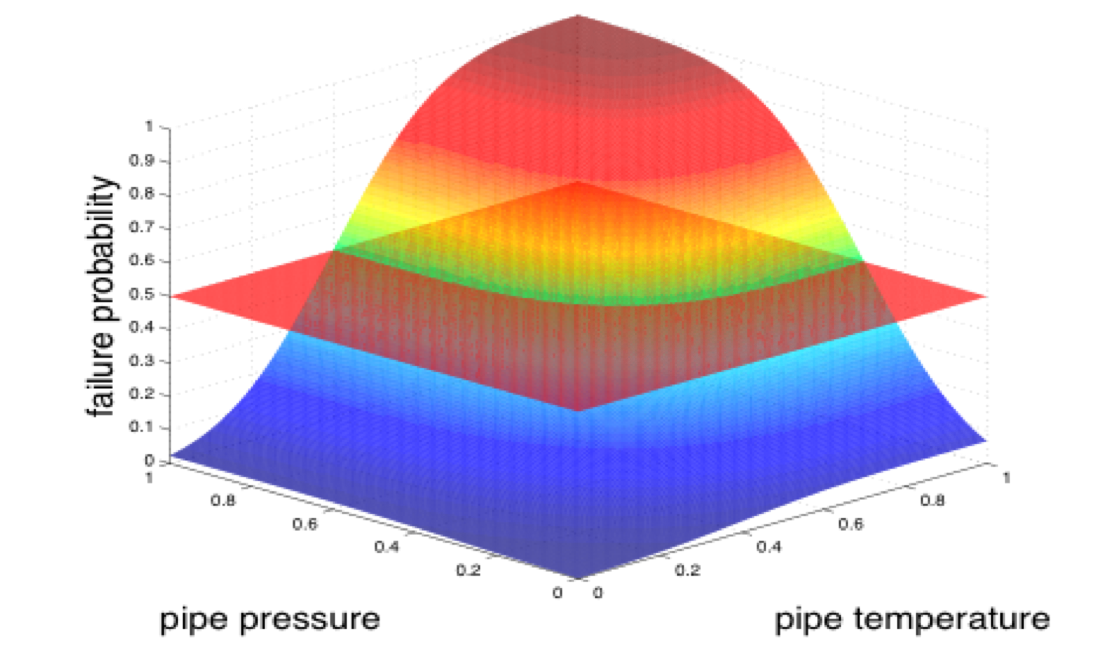
\includegraphics[width=0.5\textwidth]  {pics/NDimensionalDistributionExample.png}
  \caption{2-D CDF, function of pressure and temperature}
  \label{fig:NDDistributionExample}
\end{figure}

\subsubsection{Samplers}
The sampler performs the driving of the specific sampling strategy and, hence, determines the effectiveness of the 
analysis, from both an accuracy and computational point of view.  The samplers, available in RAVEN, can be 
categorized in three main classes:
\begin{itemize}
 \item Forward
 \item Dynamic Event Tree (DET)
 \item Adaptive
\end{itemize}
\paragraph{Forward Samplers} ~\\
The Forward sampler category collects all the strategies that perform the sampling of the input space without exploiting, 
through dynamic learning approaches, the information made available from the outcomes of calculation previously 
performed (adaptive sampling) and the common system evolution (patterns) that different sampled calculations can 
generate in the phase space (dynamic event tree).
In the RAVEN framework, several different and well-known forward samplers are available:
\begin{itemize}
\item Monte Carlo (MC)
\item Stratified based, whose most known specialization is the Latin Hyper-Cube Sampling (LHS)
\item Grid Based
\item Response Surface Design of Experiment
\item Sparse Grid
\item Factorials
\item Etc.
\end{itemize}
%%%%%%%%%%%%%%%%%%%%%%%%%%%%%%%%%%%%%%%%%%%%%%%%%%%%%%%%%%%%%%%%%%%%%%%%%%%%%%%%
\paragraph{Dynamic Event Tree Samplers}~\\
In order to clarify the idea behind the Dynamic Event Tree Sampler currently available in RAVEN, a small overview is 
needed.
\\In technologically complex systems, as nuclear power plants, an accident scenario begins with an initiating event and then 
evolves over time through the interaction of dynamics and stochastic events. This mutual action leads to the production of 
infinitely many different scenarios, which define a continuous dynamic event tree with infinite branches. At each time point, 
the stochastic variability of the accident outcomes is determined by a multivariate probability distribution. The PRA analysis 
needs an approximation to this distribution for selected consequence variables. A way to achieve this goal is an Event Tree 
approach. In dynamic PRA analysis, Conventional Event Tree sequences are run simultaneously starting from a single 
initiating event. The branches occur at user specified times and/or when an action is required by the operator and/or the 
system, creating a deterministic sequence of events based on the time of their occurrence. One of the disadvantages of 
this method is that the timing/sequencing of events and system dynamics is not explicitly accounted for in the analysis. In 
order to overcome these limitations a “dynamic” approach is needed. The Dynamic Event Tree (DET) technique brings 
several advantages, among which is the fact that it simulates probabilistic system evolution in a way that is consistent with 
the severe accident model. This leads to a more realistic and mechanistically consistent analysis of the system taken into 
consideration. The dynamic PRA, in general, and the Dynamic Event Tree methodologies in particular, are designed to 
take the timing of events explicitly into account, which can become very important especially when uncertainties in complex 
phenomena are considered. Hence, the main idea of this methodology is to let a system code determine the pathway of an 
accident scenario.
\\From an application point of view, a N-D grid is built on the CDF space. A single simulation is spawned and a set of 
triggers is added to the system code control logic. Every time a trigger gets activated (one of the CDF thresholds in the grid 
is violated), a new set of simulations (branches) is spawned. Each branch carries its own probability.
\\Figure \ref{fig:DETschemeExample} shows a practical example. In this particular case, it is assumed that the
probability failure of a pipe depends on the fluid pressure magnitude. Three probability thresholds are defined on
the cumulative distribution function. One simulation is spawned (0). As soon as the pressure of the fluid reaches a
value corresponding to a 33\% probability (CDF), a stop signal is sent and the framework starts two new
simulations (branches). The branch in which the system evolved to the newer condition (pipe failed, red line)
carries 33\% of the probability, while the other the complementary amount. The same procedure is repeated at
point 2.
\\Generally, not all the input space can be explored using a DET approach. For instance, usually the parameters affected 
by aleatory uncertainty are sampled using a dynamic event tree approach, while the ones characterized by epistemic 
uncertainty are sampled through ``forward'' sampling strategies.
\\As already mentioned, this strategy requires a tight interaction between the system code and the sampling driver (i.e., 
RAVEN framework). In addition, the system code must have a control logic capability (i.e. trigger system).  
\\In the RAVEN framework, several different DET-based samplers are available:
\begin{itemize}
\item Dynamic Event Tree (aleatory sampling);
\item Hybrid Dynamic Event Tree (aleatory and epistemic sampling);
\item Adaptive Dynamic Event Tree (goal-oriented sampling for aleatory sampling);
\item Adaptive Hybrid Dynamic Event Tree (goal-oriented sampling for aleatory and epistemic sampling).
\end{itemize}

\begin{figure}
  \centering
  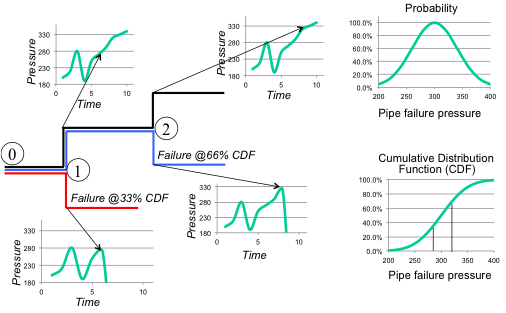
\includegraphics[width=0.7\textwidth]  {pics/DETscheme.png}
  \caption{Dynamic Event Tree simulation pattern}
  \label{fig:DETschemeExample}
\end{figure}

%%%%%%%%%%%%%%%%%%%%%%%%%%%%%%%%%%%%%%%%%%%%%%%%%%%%%%%%%%%%%%%%%%%%%%%%%%%%%%%%
\paragraph{Adaptive Samplers}~\\
A key feature available within RAVEN is the possibility to perform smart sampling (also known as adaptive sampling) as an 
alternative to classical ``forward'' techniques.
\\The motivation is that nuclear simulations are often computationally expensive, time-consuming, and high dimensional 
with respect to the number of input parameters. Thus, exploring the space of all possible simulation outcomes is unfeasible 
using finite computing resources. During simulation-based probabilistic risk analysis, it is important to discover the 
relationship between a potentially large number of input parameters and the output of a simulation using as few simulation 
trials as possible.
\\This is a typical context for performing adaptive sampling where a few observations are obtained from the simulation, a 
reduced order model (ROM) is built to represent the simulation space, and new samples are selected based on the model 
constructed. The ROM is then updated based on the simulation results of the sampled points. In this way, it is attempted to 
gain the most information possible with a small number of carefully selected sampled points, limiting the number of 
expensive trials needed to understand features of the system space.
\\In the RAVEN framework, several different adaptive samplers are available:
\begin{itemize}
\item Limit Surface Search;
\item Adaptive Dynamic Event Tree;
\item Adaptive Hybrid Dynamic Event Tree ;
\item Adaptive Sparse Grid;
\item Adaptive Sobol Decomposition.
\item Etc.
\end{itemize}


\subsubsection{Optimizers}
The optimizer performs the driving of a specific goal function over the model for value optimization. The difference between 
an optimizer and a sampler is that the former does not require sampling over a distribution, although certain specific 
optimizers may utilize stochastic approach to locate the optimal. The optimizers currently available in RAVEN can be 
categorized into the following classes:
\begin{itemize}
 \item Gradient Based Optimizer
\end{itemize}
\paragraph{Gradient Based Optimizers} ~\\
The Gradient Based Optimizer category collects all the strategies that perform the optimization based on gradient 
information, either directly provided or estimated by optimization strategy.
\\From a practical point of view, these optimization strategies represent different ways to estimate the gradient based on 
information from previously performed model evaluation.

\subsubsection{DataObject and Database}
The \textit{DataObjects'} system is a container of objects of various types that are aimed to collect the results of any RAVEN 
calculation analysis. Currently, RAVEN supports 3 different data types, each with a particular conceptual meaning:
     \begin{itemize}
        \item \textit{PointSet},  is a collection of individual objects, each describing the state of the system at a certain point 
        (e.g. in time). It can be considered a mapping between multiple sets of parameters in the input space and the resulting 
        sets of outcomes in the output space at a particular point (e.g. in time);
        \item \textit{HistorySet}, is a collection of individual objects each describing the temporal evolution of the state of the 
        system within a certain input domain. It can be considered a mapping between multiple sets of parameters in the input 
        space and the resulting sets of temporal evolution in the output space.
         \item \textit{DataSet}, is a generalization of the previously described DataObject, aimed to contain a mixture of data 
         (scalars, arrays, etc.). The variables here stored can be independent (i.e. scalars) or dependent (arrays) on certain 
         dimensions (e.g. time, coordinates, etc.). It can be considered a mapping between multiple sets of parameters in the 
         input space (both dependent and/or independent) and the resulting sets of evolution in the output space 
         (both dependent and/or independent).
     \end{itemize}
     The \textit{DataObjects}  (storage structures) represent the common ``pipe network'' among any entity in RAVEN.
\\ The Databases' system provides the capability to store and retrieve data to/from external databases (e.g. HDF5).


\subsubsection{OutStreams}
RAVEN provides the capabilities to visualize and dump out the data that are generated, imported and 
post-processed during the analysis. These capabilities are contained in the ``OutStream'' system.
 Actually, two different OutStream types are available:
 \begin{itemize}
   \item \textbf{Print}, module that lets the user dump the data contained in the internal objects;
   \item \textbf{Plot}, module aimed to provide advanced plotting capabilities.
 \end{itemize}
Both the types listed above accept as ``input'' a \textit{DataObjects} object type. 
This choice is due to the ``DataObjects'' system  having the main advantage of ensuring a standardized approach for 
exchanging the data/meta-data among the different RAVEN entities. 
Every module can project its outcomes into a DataObjects object. This provides the 
user with the capability to visualize/dump all the modules' results. 

\subsection{Steps}
The core of the RAVEN calculation flow is the Step system. 
The Step is in charge of assembling different entities in RAVEN (e.g. Samplers, Models, Databases, etc.) in order to 
perform a task defined by the kind of step being used. A sequence of 
different Steps represents the calculation flow.
\\In order to understand the information flow represented in a particular \textbf{Step}, it is
key to introduce the concept of \textit{``Role''} in a generic  \textbf{Step}. 
In the following example, a general example of a Step is shown:
\begin{lstlisting}[style=XML,morekeywords={class}]
<Simulation>
...
  <Steps>
  ...
    <StepType name='aName'>
        <Role1 class='aMainClassType' type='aSubType'>userDefinedName1</Role1> 
        <Role2 class='aMainClassType' type='aSubType'>userDefinedName2</Role2> 
        <Role3 class='aMainClassType' type='aSubType'>userDefinedName3</Role3> 
        <Role4 class='aMainClassType' type='aSubType'>userDefinedName4</Role4> 
     </StepType>
  ...
  </Steps>
...
</Simulation>
\end{lstlisting}

As shown above each \textbf{Step} consists of
a list of entities organized into \textit{``Roles''}.
%
Each role represents a behavior the entity (object) will assume during the
evaluation of the \textbf{Step}.
%
In RAVEN, several different roles are available:
\begin{itemize}
\item \textbf{Input} represents the input of the \textbf{Step}.
The allowable input objects depend on the type of \textbf{Model} in the
\textbf{Step}.
\item \textbf{Output} defines where to collect the results of an action
performed by the \textbf{Model}.
It is generally one of the following types: \textbf{DataObjects}, \textbf{Databases},
or \textbf{OutStreams}.
\item \textbf{Model} represents a physical or mathematical system or behavior.
The object used in this role defines the allowable types of
\textbf{Inputs} and \textbf{Outputs} usable in this step.
\item \textbf{Sampler or Optimizer} defines the sampling (or optimization) strategy to be used to probe the model.
\item \textbf{Function} is an extremely important role. It introduces the capability to
perform pre or post processing of Model \textbf{Inputs} and \textbf{Outputs}. Its specific
behavior depends on the \textbf{Step} is using it.
\item \textbf{ROM} defines an acceleration Reduced Order Model to use for a
\textbf{Step}.
\item \textbf{SolutionExport} represents the container of the eventual output
of a Step. For example, a \textbf{Step} is employing the
search of the Limit Surface (LS), through the class of Adaptive \textbf{Samplers}); in this case, it
contains the coordinates of the LS in the input space.
\end{itemize}
Depending on the \textbf{Step} type, different combinations of these roles can
be used.
The available steps are the following
\begin{itemize}
\item SingleRun
\item MultiRun
\item IOStep
\item RomTrainer
\item PostProcess
\end{itemize}
In order to show the information flow for a  \textbf{Step}, the  \textit{MultiRun} can be considered (being the most complex 
one). The  \textit{MultiRun} \textbf{Step} is aimed to handle calculations that involve multiple runs of a driven \textbf{Model} 
(e.g. Codes, ROMs, etc.), via a sampling or optimization strategy. 
Firstly, the RAVEN input file associates the variables to a set of PDFs and to a sampling strategy. The  \textit{MultiRun} 
step is used to perform several runs of a model (e.g. in a Monte Carlo sampling).
\begin{figure}[ht]
  \centering
  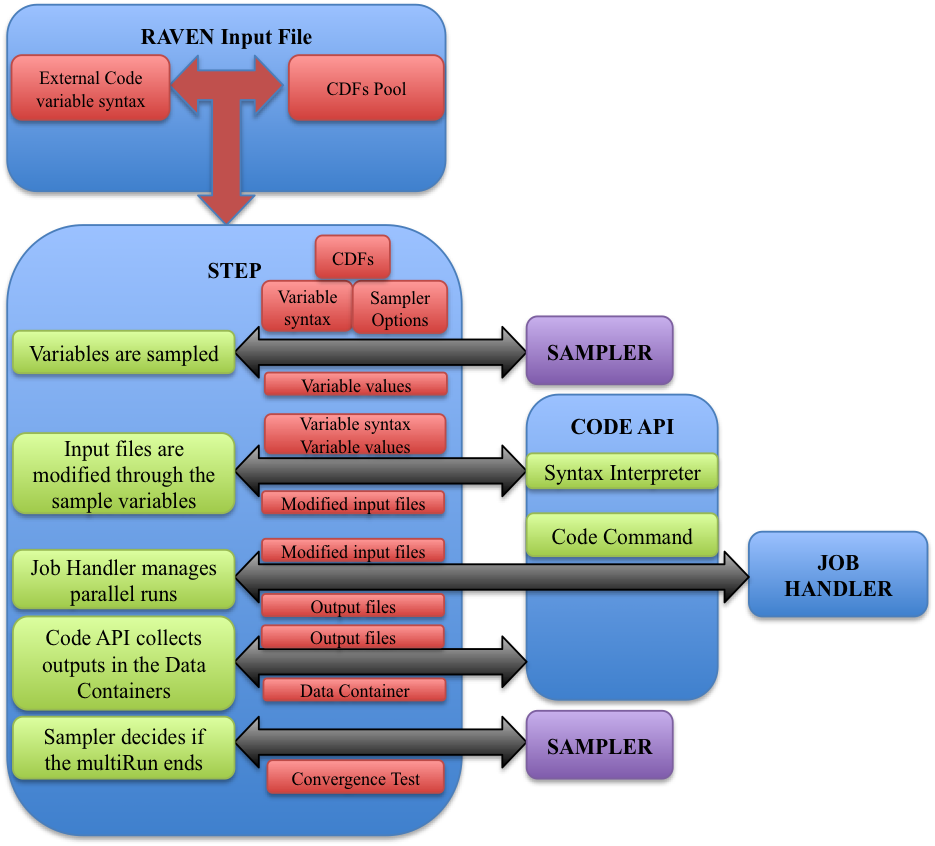
\includegraphics[width=0.8\textwidth]  {pics/MultiRunCalculationFlow.png}
  \caption{Calculation flow for a multi-run sampling}
  \label{fig:multiRun}
\end{figure}
At the beginning of each sub-sequential run, the sampler provides the new values of the variables to be perturbed. 
The \textbf{Model} API places those values in the input of the driven  \textbf{Model}  (e.g. Code, ROMs, etc.).
 At this point, the code API generates the run command and asks to be 
queued by the job handler (job scheduler). 
The job handler manages the parallel execution of as many runs as possible within a user 
prescribed range and communicates with the \textbf{Step} controller when a new set of outputs are ready to be processed. 
The \textbf{Model} API receives the new outputs and collects the data in the RAVEN internal format (\textbf{DataObjects} 
or \textbf{Databases}). The sampler is queried to assess 
if the sequence of runs is ended; if not, the  \textbf{Step}  controller asks for a new set of values 
from the sampler and the sequence 
is restarted as described in Figure~\ref{fig:multiRun}.

\subsection{Raven Input Structure}
\label{sub:InputStructure}
The RAVEN software does not have a fixed calculation flow, since all of its basic
objects can be combined in order to create a user-defined calculation flow.
%
Thus, its input (XML format) is organized in different XML blocks, each with a
different functionality.
%
The main input blocks are as follows:
\begin{itemize}
  \item \xmlNode{Simulation}: The root node containing the
  entire input, all of
  the following blocks fit inside the \emph{Simulation} block.
  %
  \item \xmlNode{RunInfo}: Specifies the calculation
  settings (number of parallel simulations, etc.).
  %
  \item \xmlNode{Files}: Specifies the files to be
  used in the calculation.
  %
  \item \xmlNode{Distributions}: Defines distributions
  needed for describing parameters, etc.
  %
  \item \xmlNode{Samplers}: Sets up the strategies used for
  exploring an uncertain domain.
  %
  \item \xmlNode{Optimizers}: Sets up the strategies used for
  minimizing/maximizing an objective function.
  %
  \item \xmlNode{DataObjects}: Specifies internal data objects
  used by RAVEN.
  %
  \item \xmlNode{Databases}: Lists the HDF5 databases used
  as input/output to a
  RAVEN run.
  %
  \item \xmlNode{OutStreams}: Visualization and
  Printing system block.
  %
  \item \xmlNode{Models}: Specifies codes, ROMs,
  post-processing analysis, etc.
  %
  \item \xmlNode{Functions}: Details interfaces to external
  user-defined functions and modules.
  %
  the user will be building and/or running.
  %
  \item \xmlNode{Steps}: Combines other blocks to detail a
  step in the RAVEN workflow including I/O and computations to be performed.
  %
\end{itemize}

Each of these blocks are explained in dedicated sections in the user manual ~\cite{RAVENuserManual}.
%




\subsection{Data Design and Control}
The data transfer in the RAVEN software is fully standardized:
\begin{itemize}
  \item  \textbf{\textit{Input}}: API deployed by Code Interfaces and/or Model APIs;
  \item \textbf{\textit{Output}}: API deployed by the \textbf{DataObjects}  and \textbf{Databases}.
\end{itemize}
The documentation of these APIs is reported in the RAVEN user manual (\cite{RAVENuserManual})

\subsection{Human-Machine Interface Design} 
 There are no human system integration requirements associated with this software.
 \subsection{System Interface Design} 
RAVEN does not own any physical model. For this reason, it needs to be interfaced with external
or user input-defined
software representing the engine for simulating physical models (systems). 
The interface with external systems in the RAVEN software is fully standardized via clear APIs deployed by
 the \textbf{Models} entities.
The documentation of these APIs is reported in the RAVEN user manual (\cite{RAVENuserManual})

 \subsection{Security Structure} 
The software is accessible to the open-source community (Apache License, Version 2.0). No restrictions for downloading or redistributing is applicable.

 \section{REQUIREMENTS CROSS-REFERENCE} 
The requirements are detailed in SPC-2366, ``RAVEN Software Requirements Specification (SRS) and Traceability Matrix''.



    % ---------------------------------------------------------------------- %
    % References
    %

\addcontentsline{toc}{section}{References}
\bibliographystyle{ieeetr}
\bibliography{raven_software_design_description}

\section*{Document Version Information}

d317572ffb80f564d27ec54e5db24d763705a8a5 Aaron Epiney - INL Tue, 17 Oct 2017 XX:XX:XX -0600


\end{document}
